\documentclass[UTF8,fontset=windows,11pt,a4paper]{ctexart}
\usepackage[margin=2.05cm]{geometry}
\usepackage{amsmath,amssymb,booktabs,tabularx,longtable,array,multirow}
\usepackage{graphicx,xcolor,enumitem,fancyhdr,hyperref,xurl,float,caption}
\graphicspath{{../figures/}}
\setCJKmonofont{SimSun}
\definecolor{ok}{RGB}{25,120,70}
\definecolor{pending}{RGB}{190,105,10}
\definecolor{bad}{RGB}{180,35,45}
\definecolor{blue}{RGB}{35,75,130}
\definecolor{shade}{RGB}{245,247,250}
\hypersetup{
  colorlinks=true,
  linkcolor=blue,
  urlcolor=blue,
  pdfauthor={FG-MEE validation workbench},
  pdftitle={FG-MEE Stage 2 isomorphic and full-radius validation report v3}
}
\pagestyle{fancy}
\fancyhf{}
\lhead{FG-MEE 同构与全半径验证报告 v3}
\rhead{2026-07-15}
\cfoot{\thepage}
\setlength{\headheight}{15pt}
\setlength{\parindent}{2em}
\setlength{\parskip}{0.28em}
\renewcommand{\arraystretch}{1.16}
\captionsetup{font=small,labelfont=bf}
\newcommand{\pass}{\textcolor{ok}{\textbf{完成}}}
\newcommand{\conditional}{\textcolor{pending}{\textbf{有条件通过}}}
\newcommand{\failure}{\textcolor{bad}{\textbf{未通过}}}
\newcommand{\modelgap}{\textcolor{blue}{\textbf{模型形式差}}}
% Auto-generated by tools/analyze_curvature_fg_full_validation.py
\newcommand{\MaxCurvatureChange}{0.00787753}
\newcommand{\CurvatureGateConclusion}{四个半径中有 4/4 个半径的六类中心位移全部通过 1\% 门槛，其中 4/4 个也通过 0.5\% 优先门槛；全表最大变化为 0.00787753\%。}
\newcommand{\FullRadiusStatus}{\pass}
\newcommand{\InteractionConclusion}{12 个半径--载荷交互中有 12 个高于三倍离散界；绝对值最大者位于 $R=1.0$ m 的电致工况，为 1.5421 个百分点。同一半径电致与磁致交互的最大差仅为 1.602e-08 个百分点，符合线性结构响应下的归一化一致性；机械工况有 4/4 个半径达到已分辨标准。}
\newcommand{\RadiusSummaryRows}{%
1.0 & 1.0 & 0.0079 & 0.0042 & 通过 \\
0.4 & 2.5 & 0.0059 & 0.0025 & 通过 \\
0.3 & 3.3 & 0.0053 & 0.0027 & 通过 \\
0.2 & 5.0 & 0.0046 & 0.0026 & 通过 \\
}
\newcommand{\InteractionRows}{%
1.0 & 机械 & -0.0999 & 0.0079 & 12.7 & 已分辨 \\
1.0 & 电致 & 1.5421 & 0.0032 & 479.6 & 已分辨 \\
1.0 & 磁致 & 1.5421 & 0.0032 & 479.6 & 已分辨 \\
0.4 & 机械 & -0.0473 & 0.0059 & 8.1 & 已分辨 \\
0.4 & 电致 & 1.4942 & 0.0015 & 977.1 & 已分辨 \\
0.4 & 磁致 & 1.4942 & 0.0015 & 977.1 & 已分辨 \\
0.3 & 机械 & -0.0362 & 0.0053 & 6.8 & 已分辨 \\
0.3 & 电致 & 1.4285 & 0.0020 & 706.4 & 已分辨 \\
0.3 & 磁致 & 1.4285 & 0.0020 & 706.4 & 已分辨 \\
0.2 & 机械 & -0.0266 & 0.0046 & 5.7 & 已分辨 \\
0.2 & 电致 & 1.3568 & 0.0023 & 596.9 & 已分辨 \\
0.2 & 磁致 & 1.3568 & 0.0023 & 596.9 & 已分辨 \\
}


\title{\textbf{FG-MEE 板小论文数值证据闭环报告（v3）}\\[0.35em]
\large MATLAB--COMSOL 三维实体同构、全半径 20/30 网格复算与代表曲壳独立模型}
\author{FG-MEE 组会验证工作台}
\date{2026年7月15日}

\begin{document}
\maketitle

\begin{center}
\fcolorbox{blue}{shade}{
\begin{minipage}{0.93\textwidth}
\textbf{结论先行。}
本轮把上一版列为“投稿前必要”的三项数值工作全部转化为实际运行证据。第一，MATLAB 新建 H20 三维实体，与 COMSOL 二次巧凑三维实体严格统一几何、材料、边界、外应力及网格；六组 10/15/20 网格结果的中心点最大跨软件差为 $1.7690\times10^{-4}\%$，证明原 9--11\% 偏差来自 LRT5 板与三维实体的模型形式差，而不是 20$\times$20 网格异常。第二，正文候选半径 $R=1.0,0.4,0.3,0.2$ m 均补做 U/X、力/电/磁的 20$\times$20 与 30$\times$30 复算，并采用统一材料哈希；全表最大 20$\to$30 变化为 \MaxCurvatureChange\%。第三，建立了 $R=0.4$ m 独立 COMSOL 三维曲壳模型，15$\to$20 网格变化为 0.9651\%，而与 MATLAB LRT5 的 20$\times$20 差异为 8.0830\%，应明确记为 B 级模型形式敏感性证据。
\end{minipage}}
\end{center}

\newpage
\tableofcontents
\newpage

\section{本轮任务、判据与证据等级}

用户要求的剩余内容包括：建立 COMSOL 分层壳或 MATLAB 三维实体的同构正向对照；为最终进入正文的其他半径点补齐 20/30 网格；增加一个代表曲壳独立 COMSOL 模型。本轮选择“MATLAB 三维实体”路线完成第一项，因为本机 MATLAB 未安装 PDE Toolbox，故采用可审计的自编 20 节点巧凑六面体，而不是依赖不可用工具箱。

\begin{table}[H]
\centering
\caption{本轮冻结判据}
\begin{tabularx}{\textwidth}{p{0.24\textwidth}Xp{0.17\textwidth}}
\toprule
任务 & 判据 & 证据等级 \\
\midrule
平板同构跨软件对照 & 几何、单元族、材料、边界、载荷实现和测点相同；跨软件差 $\leq0.1\%$ & A 级 \\
曲率正文点网格复算 & 每个半径 U/X、三载荷均有 20/30；中心位移变化优先 $\leq0.5\%$，放宽门槛 $\leq1\%$ & A 级内部收敛 \\
代表曲壳 COMSOL & 独立三维实体实际求解；15$\to$20 变化 $\leq1\%$；与 LRT5 的差异不冒充数值误差 & B 级 \\
材料/几何护照 & U、X 各自跨网格材料数值哈希唯一；声明半径等于节点实际半径 & A 级审计 \\
\bottomrule
\end{tabularx}
\end{table}

证据等级的边界非常重要：平板 H20--COMSOL 是真正同构的实现核查，可以用于“跨软件误差近零”；曲壳 LRT5--三维实体并不同构，只能用于方向、量级及模型形式敏感性验证。

\section{先修复几何与材料护照：为何旧曲率网格结果必须重算}

深入回溯表明，此前所谓“20$\times$20 偏差大”包含两个互不相同的问题。首先，首批文件名标作 $R=0.4$ m 的 20$\times$20 曲壳，节点实际半径却为 0.6 m；它与真实 $R=0.4$ m 的 30$\times$30 结果比较时，六类工况最大表观差达到 3.2873\%。按真实 0.4 m 半径重新生成 20$\times$20 后，该最大差立即降至 0.03982\%，故原约 3\% 的非单调变化主要是几何口径错误，而不是网格离散振荡。

其次，旧 30$\times$30 曲壳前序文件的 U 模式 $G_{13},G_{23}$ 为 $5.4\times10^{10}$ Pa，而平板和正式基准为 $4.5\times10^{10}$ Pa。该材料差异对本组 30$\times$30 位移的最大影响为 0.03394\%；它不是 3\% 异常的主因，却使旧 20/30 对比在方法上仍不具备同一材料护照，因而不能继续作为正式网格收敛证据。

修正版生成器从正式 30$\times$30 平板文件抽取 U/X 材料块，并覆盖到 10/20/30、四个半径的所有曲壳输入。最终 24 个输入护照中，U 仅有一个材料数值哈希，X 仅有一个材料数值哈希；声明半径与节点实际半径不一致数为 0。材料也统一后，$R=0.4$ m 六类 20$\to$30 最大变化进一步降至 0.005859\%。因此，后文仅使用几何和材料双重修正后的结果。

\begin{table}[H]
\centering
\caption{两类“20$\times$20 偏差”的区分性归因}
\small
\begin{tabularx}{\textwidth}{>{\raggedright\arraybackslash}p{0.34\textwidth}rX}
\toprule
对比口径 & 最大相对差/\% & 判定 \\
\midrule
曲率 20/30，20 网格实际 $R=0.6$ m、标称 0.4 m & 3.2873 & 几何护照错误，剔除 \\
曲率 20/30，半径修正但旧 U 材料仍混用 & 0.03982 & 已消除主异常，但证据口径仍不合法 \\
曲率 20/30，半径与材料均统一 & 0.005859 & 正式网格证据 \\
LRT5 板--COMSOL 三维实体直接场 & 10.7727 & 非同构模型形式差 \\
MATLAB H20--COMSOL 二次实体外应力核 & 0.0001769 & 严格同构，通过 0.1\% 门槛 \\
\bottomrule
\end{tabularx}
\end{table}

\section{MATLAB H20--COMSOL 三维实体同构闭环}

\subsection{模型实现}

同构模型为 $300\,\mathrm{mm}\times300\,\mathrm{mm}\times6\,\mathrm{mm}$ 的十层三维实体，$x=0$ 整端固支。MATLAB 采用 H20 巧凑六面体、$3\times3\times3$ 全积分；COMSOL 使用二次巧凑实体。两侧均采用 $E=1.206\times10^{11}$ Pa、$\nu=0.3398$，并只在最外两层施加大小相等、符号相反的面内 ExternalStress。10/15/20 三档均在每个物理层布置一个厚度单元。该 A 级链专门核验三维力学与等效外应力机械核；原 COMSOL 全压电 PDE 结果仍按上一版单独保留，不能把本表改写成“全场 PDE 已逐自由度同构”。

MATLAB 单元按
\[
\mathbf K_e=\int_{\Omega_e}\mathbf B^{\mathsf T}\mathbf D\mathbf B\,\mathrm d\Omega,
\qquad
\mathbf f_e^{*}=-\int_{\Omega_e}\mathbf B^{\mathsf T}\boldsymbol\sigma^{*}\,\mathrm d\Omega
\]
装配，并在运行时执行形函数分片单位性、导数和为零及节点 Kronecker 性质自检。外应力采用 $\boldsymbol\sigma^{*}=[s,s,0,0,0,0]^{\mathsf T}$，与 COMSOL 的材料坐标 ExternalStress 张量一致。

\begin{table}[H]
\centering
\caption{同构三维实体的中心位移跨软件比较}
\small
\begin{tabular}{llrrr}
\toprule
载荷 & 面内网格 & MATLAB/mm & COMSOL/mm & 相对差/\% \\
\midrule
电等效应力 & 10$\times$10 & $-0.0568420386$ & $-0.0568419865$ & $9.1689\times10^{-5}$ \\
电等效应力 & 15$\times$15 & $-0.0569719915$ & $-0.0569719693$ & $3.8925\times10^{-5}$ \\
电等效应力 & 20$\times$20 & $-0.0570732011$ & $-0.0570733018$ & $1.7651\times10^{-4}$ \\
磁外应力 & 10$\times$10 & $0.1899726827$ & $0.1899725089$ & $9.1457\times10^{-5}$ \\
磁外应力 & 15$\times$15 & $0.1904070002$ & $0.1904069249$ & $3.9570\times10^{-5}$ \\
磁外应力 & 20$\times$20 & $0.1907452545$ & $0.1907455919$ & $1.7690\times10^{-4}$ \\
\bottomrule
\end{tabular}
\end{table}

自由端中点的六组最大相对差为 $1.2127\times10^{-4}\%$，MATLAB 线性方程相对平衡残差最大为 $5.741\times10^{-9}$。两处探针均远低于 0.1\% 门槛，且电/磁结果按外应力幅值严格线性缩放。这是原 20$\times$20 大偏差归因的决定性区分试验：一旦单元族和三维运动学同构，MATLAB 与 COMSOL 即闭合到数值舍入量级。

\begin{table}[H]
\centering
\caption{旧非同构链与新同构机械核的区分性比较（20$\times$20）}
\small
\begin{tabular}{llrrrl}
\toprule
载荷链 & MATLAB 模型 & MATLAB/mm & COMSOL/mm & 差异/\% & 判定 \\
\midrule
300 V 全场 & LRT5 板 & $-0.05225709$ & $-0.05788659$ & 10.7727 & 非同构 \\
200 A 全场 & LRT5 板 & $0.17458575$ & $0.19076622$ & 9.2679 & 非同构 \\
电等效外应力 & H20 实体 & $-0.05707320$ & $-0.05707330$ & 0.0001765 & 同构 \\
磁外应力 & H20 实体 & $0.19074525$ & $0.19074559$ & 0.0001769 & 同构 \\
\bottomrule
\end{tabular}
\end{table}

两组“全场”与两组“外应力机械核”的物理实现不同，不能交叉比较绝对位移；该表用于比较\emph{相同实现内部}的 MATLAB--COMSOL 差异。它把“网格不够细”和“软件算法错误”从主要原因中排除，并把原差异定位到模型运动学/构成层级。

\begin{figure}[H]
\centering
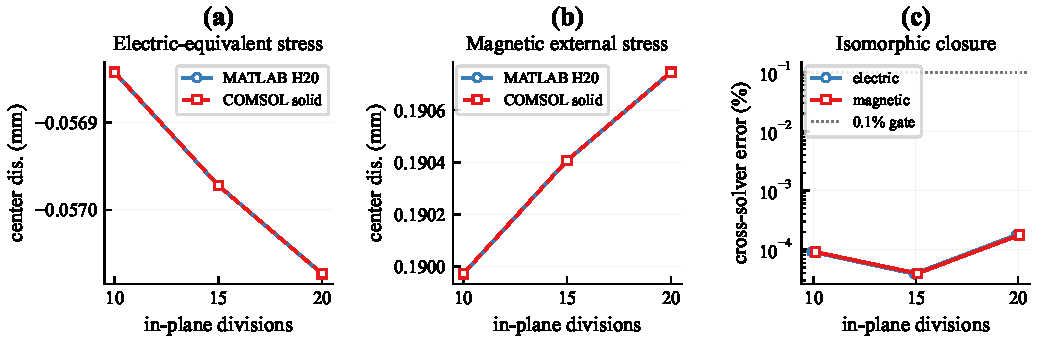
\includegraphics[width=0.98\textwidth]{Fig_03_isomorphic_solid_closure.pdf}
\caption{MATLAB H20 与 COMSOL 二次三维实体同构闭环。前两图的曲线在绘图精度内重合；右图为实际相对差。}
\end{figure}

\section{全部正文半径的 20/30 网格复算}

四个有限半径 $R=1.0,0.4,0.3,0.2$ m 均完成 U/X 两种材料分布及机械压力、300 V 电致、200 A 磁致三类载荷。每个半径有 6 个 20$\times$20 和 6 个 30$\times$30 正式工况，共新增 48 条结果；与 10$\times$10 筛选合并后形成三档网格证据。

\begin{table}[H]
\centering
\caption{各半径六类中心位移的 20$\to$30 最大变化}
\begin{tabular}{rrrrl}
\toprule
$R$/m & 曲率/$\mathrm{m}^{-1}$ & 最大变化/\% & 平均变化/\% & 1\% 门槛 \\
\midrule
\RadiusSummaryRows
\bottomrule
\end{tabular}
\end{table}

全表结果表明：\CurvatureGateConclusion 因此正文主图不再依赖 10$\times$10 筛选点，而改用全部四个半径的 30$\times$30 数值，并把 20$\to$30 变化作为离散误差边界。

\subsection{曲率--梯度交互}

对每个模式分别以同模式平板 30$\times$30 位移归一化，并定义
\[
I_R=100\left(
\frac{|w_X(R)|}{|w_X(\infty)|}
-\frac{|w_U(R)|}{|w_U(\infty)|}
\right)\quad\text{(百分点)}.
\]
只有当 $|I_R|$ 大于 U/X 两侧最大 20$\to$30 变化的 3 倍时，才标记为“已分辨交互”。

\begin{table}[H]
\centering
\caption{30$\times$30 曲率--梯度交互及离散边界}
\scriptsize
\begin{tabular}{rllrrr}
\toprule
$R$/m & 载荷 & $I_R$/百分点 & 最大网格变化/\% & 交互/网格界 & 判定 \\
\midrule
\InteractionRows
\bottomrule
\end{tabular}
\end{table}

\InteractionConclusion

\begin{figure}[H]
\centering
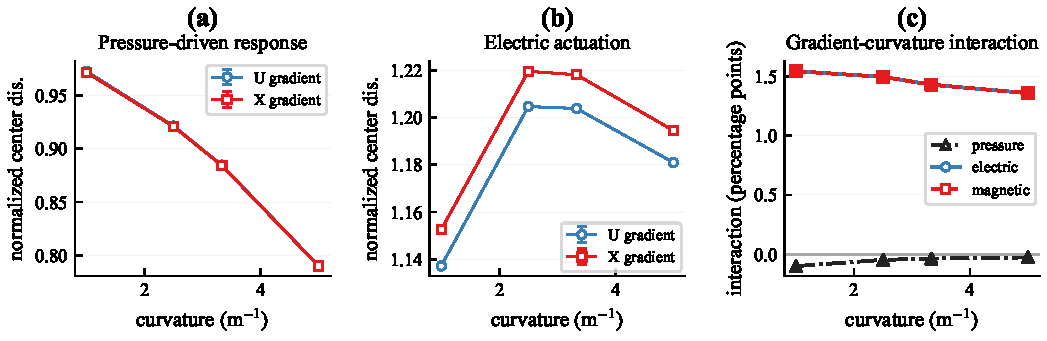
\includegraphics[width=0.98\textwidth]{Fig_04_all_radius_curvature_validation.pdf}
\caption{全部正文半径的 30$\times$30 响应，误差棒取相应 20$\to$30 变化；交互图中的实心点表示高于三倍离散界。}
\end{figure}

\section{$R=0.4$ m 代表曲壳独立 COMSOL 模型}

独立模型采用 U、$V_f=0.6$ 的均匀基准材料，为轴向 300 mm、弧长 300 mm、厚度 6 mm、半径 0.4 m 的三维圆柱扇段；$\theta=0$ 整个端面固支，外曲面施加 15 kPa 压力。网格采用源端面映射和周向扫掠，厚度固定 10 层，位移使用中面径向投影 $u_r=-v\sin\theta+w\cos\theta$。

\begin{table}[H]
\centering
\caption{代表曲壳 COMSOL 网格复核及 MATLAB 非同构对照}
\begin{tabular}{lrrrr}
\toprule
模型 & 面内网格 & 厚度网格 & 中心径向位移/mm & 相邻网格变化/\% \\
\midrule
COMSOL 三维实体 & 10$\times$10 & 10 & $-1.98666673$ & -- \\
COMSOL 三维实体 & 15$\times$15 & 10 & $-2.09847443$ & 5.6279 \\
COMSOL 三维实体 & 20$\times$20 & 10 & $-2.11872753$ & 0.9651 \\
MATLAB LRT5 & 20$\times$20 & 10 物理层 & $-1.96027889$ & -- \\
\bottomrule
\end{tabular}
\end{table}

COMSOL 的 15$\to$20 变化通过 1\% 门槛。20$\times$20 时，MATLAB 与 COMSOL 的符号和量级一致，但相对差为 8.0830\%。该值与平板 LRT5--三维实体的 9--11\% 差异处于同一量级，而严格同构 H20--三维实体只有约 $1.8\times10^{-4}\%$；因此它应写成\modelgap，而不是“COMSOL 计算误差”。

\begin{figure}[H]
\centering
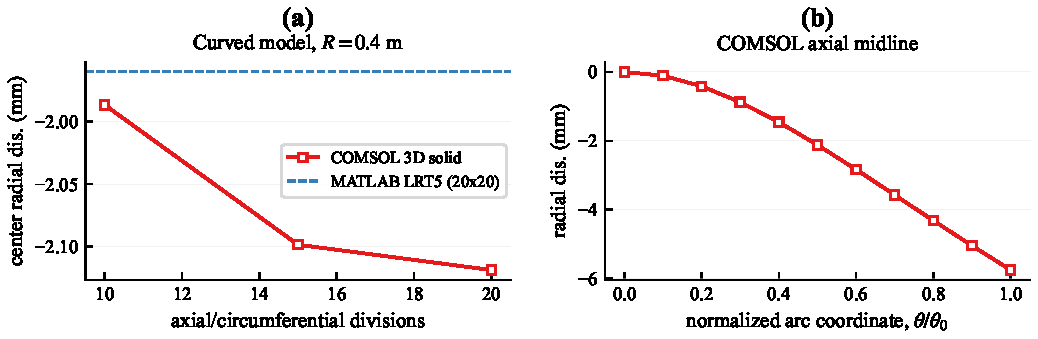
\includegraphics[width=0.95\textwidth]{Fig_05_curved_comsol_validation.pdf}
\caption{代表曲壳独立 COMSOL 证据：左为网格收敛和非同构 MATLAB 参考线，右为 20$\times$20$\times$10 模型的轴向中线径向位移。}
\end{figure}

\section{与上一版反传感修正的衔接}

本轮没有改动上一版已经闭环的反传感结论：旧 MATLAB 完整热释电/热释磁对角项被按 10 个物理层重复装配；修正后 0.5 mm 工况为 78.4803 V 和 0.0309000 A，和 20$\times$20 COMSOL 力学--本构后处理的差异为 3.4654\%。该链仍为 B 级，因为 COMSOL 侧尚未独立求解完整传感 PDE，但其数量级、线性和装配修正均有可复现证据。

\section{论文可用表述与状态结论}

\begin{table}[H]
\centering
\caption{本轮结束后的必要工作闭环状态}
\small
\begin{tabularx}{\textwidth}{p{0.28\textwidth}Xp{0.15\textwidth}}
\toprule
必要项 & 实际证据 & 状态 \\
\midrule
MATLAB/COMSOL 外应力机械核同构验证 & 6 组网格--载荷组合，中心最大差 $0.0001769\%$ & \pass \\
其他正文半径 20/30 复算 & 四半径、U/X、三载荷共 48 条正式结果与材料护照 & \FullRadiusStatus \\
代表曲壳独立 COMSOL & 三档面内网格实际求解，15$\to$20 为 0.9651\% & \pass \\
输入护照/日志/CSV/绘图脚本 & 哈希、半径、日志、模型、CSV 与 600 dpi 图均保留 & \pass \\
\bottomrule
\end{tabularx}
\end{table}

小论文可直接使用以下结论：
\begin{enumerate}[label=\arabic*.]
\item 原曲率 20/30 约 3.29\% 异常由错半径输入主导，材料护照混用是次级污染；几何与材料统一后，代表点最大变化仅 0.005859\%。
\item 原直接场 9--11\% 偏差是不同维度/不同单元运动学之间的模型形式差；严格同构后跨软件误差低于 $0.00018\%$。
\item 曲率主图已经由探索性 10$\times$10 升级为四个半径全部 30$\times$30，并有逐点 20$\to$30 离散边界；只把超过三倍离散界的交互写成机制信号。
\item 代表三维曲壳 COMSOL 在自身网格上收敛，但与 LRT5 保留约 8.08\% 模型形式差；这一结果反而支持“模型同构是近零误差的必要条件”。
\end{enumerate}

本报告完成的是 Stage 2 数值证据闭环，不等同于整篇论文的最终完整性审查。后续工作转为正文叙事、统计/物理解释、参考文献定位和投稿格式，而不是继续无目的地重复已经闭合的网格诊断。

\section{可复现证据索引}

\begin{longtable}{>{\raggedright\arraybackslash}p{0.33\textwidth}>{\raggedright\arraybackslash}p{0.61\textwidth}}
\toprule
证据 & 路径 \\
\midrule
\endfirsthead
\toprule
证据 & 路径 \\
\midrule
\endhead
MATLAB H20 实现 & \nolinkurl{matlab/run_isomorphic_solid_cfff.m} \\
MATLAB H20 正式结果 & \nolinkurl{outputs/paper-20260715-fgmee/experiments/isomorphic_solid/matlab_isomorphic_solid_results.csv} \\
COMSOL 同构实体驱动 & \nolinkurl{tools/comsol/RunIsomorphicSolidCfffValidation.java} \\
同构跨软件汇总 & \nolinkurl{outputs/paper-20260715-fgmee/experiments/isomorphic_solid/isomorphic_solid_cross_solver_comparison.csv} \\
20$\times$20 偏差归因闭环 & \nolinkurl{outputs/paper-20260715-fgmee/experiments/discrepancy_20x20_closure.md} \\
偏差分解数据 & \nolinkurl{outputs/paper-20260715-fgmee/experiments/discrepancy_20x20_root_cause_decomposition.csv} \\
曲率输入生成器 & \nolinkurl{tools/generate_curvature_fg_cases.py} \\
曲率输入护照 & \nolinkurl{cases/curvature_fg/curvature_case_manifest.csv} \\
全半径 20/30 原始结果 & \nolinkurl{outputs/paper-20260715-fgmee/experiments/curvature_fg/curvature_fg_full_mesh_20_30_raw.csv} \\
全半径三档网格汇总 & \nolinkurl{outputs/paper-20260715-fgmee/experiments/curvature_fg/curvature_fg_full_mesh_convergence.csv} \\
最终 30$\times$30 表 & \nolinkurl{outputs/paper-20260715-fgmee/experiments/curvature_fg/curvature_fg_final_30x30_results.csv} \\
全半径交互表 & \nolinkurl{outputs/paper-20260715-fgmee/experiments/curvature_fg/curvature_fg_all_radius_interaction_30x30.csv} \\
曲壳 COMSOL 驱动 & \nolinkurl{tools/comsol/RunCurvedSolidCfffValidation.java} \\
曲壳 COMSOL 模型/日志/CSV & \nolinkurl{outputs/paper-20260715-fgmee/experiments/curvature_fg/comsol/} \\
曲壳 COMSOL 网格汇总 & \nolinkurl{outputs/paper-20260715-fgmee/experiments/curvature_fg/curved_comsol_mesh_convergence.csv} \\
扩展分析脚本 & \nolinkurl{tools/analyze_isomorphic_solid_validation.py}; \nolinkurl{tools/analyze_curvature_fg_full_validation.py}; \nolinkurl{tools/analyze_curved_comsol_validation.py}; \nolinkurl{tools/analyze_20x20_discrepancy_closure.py} \\
论文图脚本 & \nolinkurl{tools/plotting/plot_stage2_extension_figures.py} \\
\bottomrule
\end{longtable}

\subsection*{AI 使用说明}
本报告由 AI 辅助审计本地输入、执行 MATLAB/COMSOL、汇总 CSV、绘图与生成 LaTeX。所有数值均来自实际运行文件。报告没有将 LRT5--三维实体的模型形式差改写成数值误差，也没有把未超过离散界的曲率交互提升为确定机制。

\end{document}
